Avant de vouloir résoudre notre problème du modèle partiellement linéaire, nous allons d'abord nous intéresser à l'estimation non paramétrique lorsque l'on dispose de données avec erreur de mesure dans les covariables. Considérons donc le modèle de données suivant :

\begin{equation}
    \begin{cases}
        Y = m(Z) + \varepsilon
        \\
        \varepsilon \indep Z
        \\
        \esperancesachant Z \varepsilon = 0
    \end{cases}
\end{equation}

avec le modèle d'observation suivant :

\begin{equation}
    \begin{cases}
        \left( \zei, \yi \right)_{i \in \intervaleint 1 n}
        \\
        \zei = \zi + \vi 
        \\
        V \indep Z
    \end{cases}
\end{equation}

La méthode de lissage non paramétrique à noyaux classique ne peut plus marcher car le bruit dans la covariable perturbe l'information et un moyennage local introduirait un biais non négligeable :

\begin{figure}[H]
    \centering
    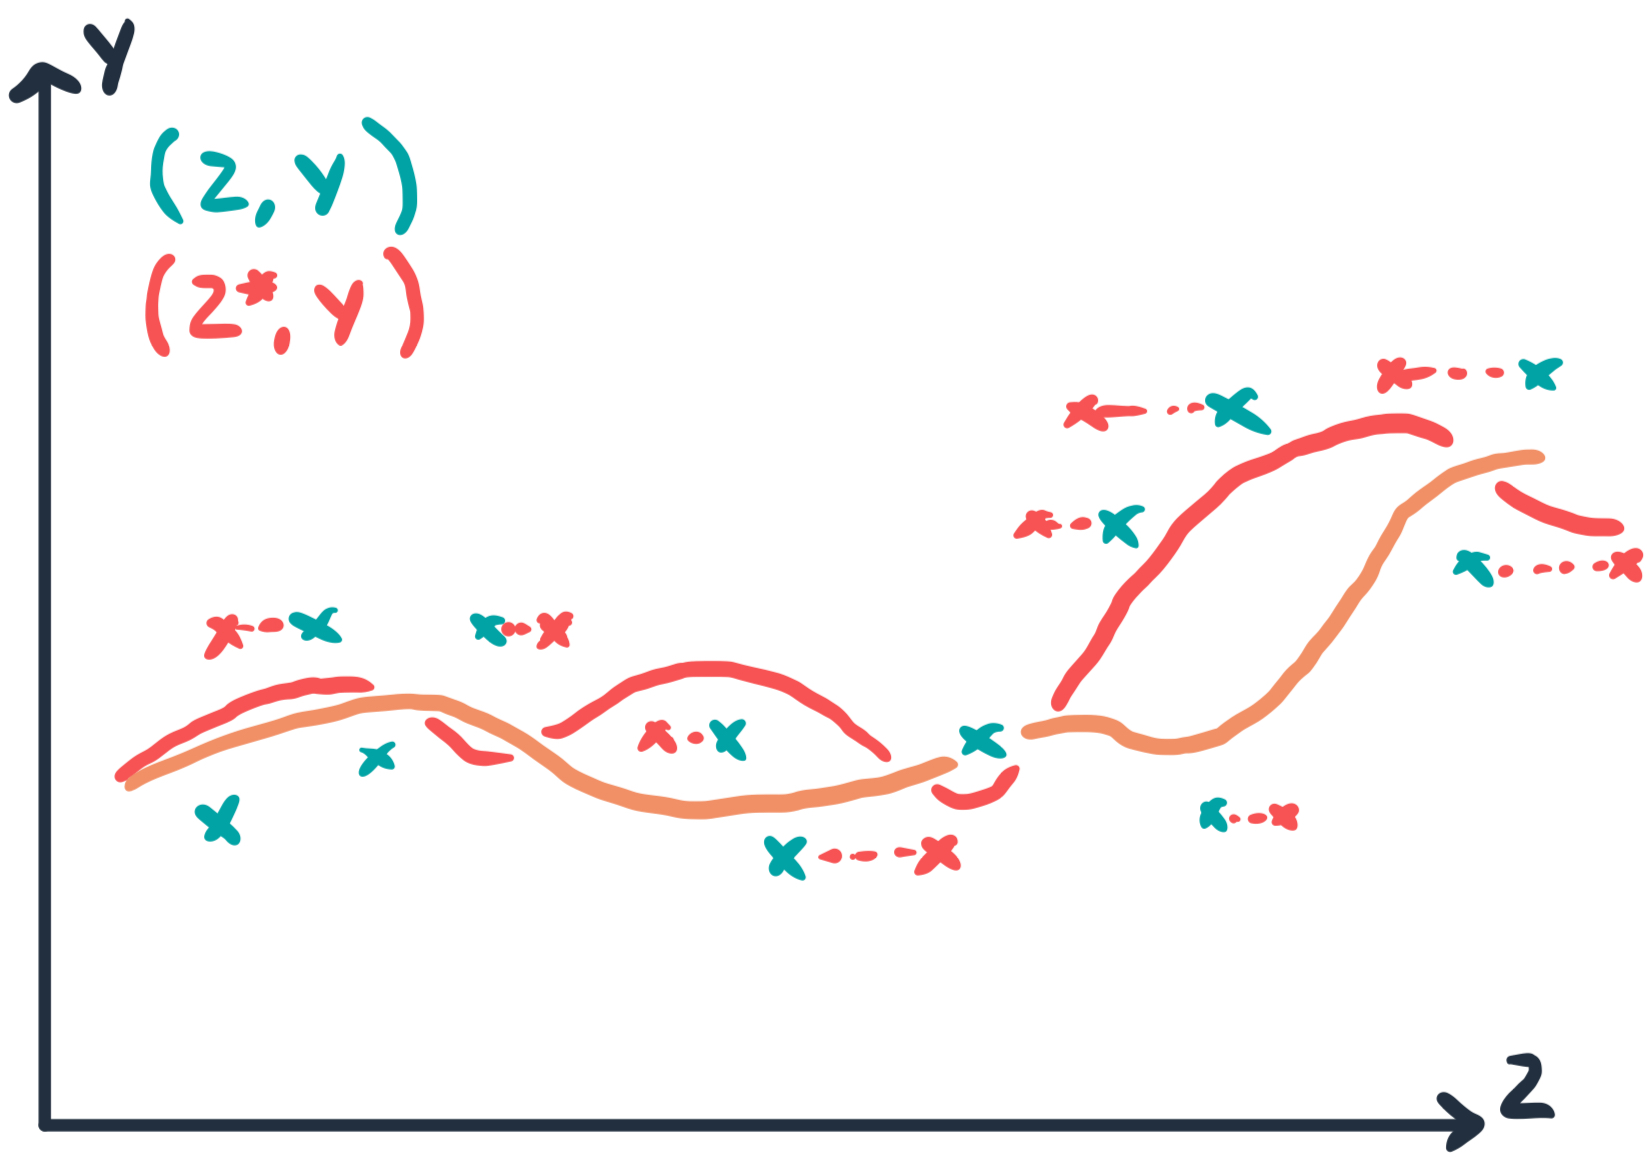
\includegraphics[width=0.35\textwidth]{Images/noyaux_erreur.jpeg}
    \caption{Lissage non paramétrique à noyaux avec erreur de mesure dans les covariables sans prise en compte de l'erreur.}
    \label{fig:noyaux_erreur}
\end{figure}

L'estimateur de Nadaraya-Watson de la fonction $m$ est un estimateur que l'on pourrait interpréter comme un estimateur plug-in utilisant l'estimation de la densité conditionnelle de $Y$ sachant $Z$ à partir de l'estimateur de la densité de $Z$ et de la densité jointe de $(Z,Y)$. Sauf que la densité que nous observons est celle de $(Z+V,Y)$ et non celle de $(Z,Y)$. L'erreur $V$ étant indépendante de $Z$, la densité de $Z+V$ est la convolution des deux densités :

\begin{equation}
    f_{Z+V} = \convo{f_Z}{f_V}
\end{equation}

La convolution de fonctions intégrables est une opération qui a été étudiée massivement dû à ses nombreuses applications. Elle se comporte algébriquement bien dans le monde fréquentiel : en effet la transformée de Fourier d'une convolution et le produit des transformées de Fourier

\begin{equation}
	\mathcal F \convo f g = \mathcal F[f] \times \mathcal F [g]
\end{equation}

On aimerait à partir de nos données observées avec erreur de mesure dans les covariables, utiliser un lissage à noyau qui ne prendrait en compte que l'information dans les covariables. En d'autre termes juste prendre l'information de $f_Z$ dans $f_{Z+V}$. En se ramenant dans le monde fréquentiel, on remarque que : 

\begin{align}
    \mathcal F \left[ f_{Z+V} \right] &= \mathcal F \left[ f_Z \right] \times \mathcal F \left[ f_V \right] \notag
    \\
    \mathcal F \left[ f_Z \right] &= \frac{\mathcal F \left[ f_{Z+V} \right]}{\mathcal F \left[ f_V \right]}
    \\
    \inverse{\mathcal F} \left( \mathcal F \left[ f_Z \right] \right) &=  \inverse{\mathcal F} \left( \frac{\mathcal F \left[ f_{Z+V} \right]}{\mathcal F \left[ f_V \right]} \right) \notag
    \\
    f_Z &= \inverse{\mathcal F} \left( \frac{\mathcal F \left[ f_{Z+V} \right]}{\mathcal F \left[ f_V \right]} \right)
\end{align}

C'est ce qui va venir motiver l'ensemble de la méthodlogie qui sera exposée dans la suite de cette section : on appelle ainsi naturellement cette opération \emph{\og la déconvolution \fg}.
Si la transformée de Fourier semble être un outil obscur pour le statisticien, il n'en est rien. Le statisticien a probablement utilisé à nombreuses reprises la transformée de Fourier sans le savoir.

\begin{definition}[Transformée de Fourier]
    Soit $f : \grandR \rightarrow \grandR$ une fonction intégrable.
    On appelle transformée de Fourier de $f$ la fonction $\varphi_f$ définie par :

    \begin{equation*}
        \varphi_f : \func
        {\grandR}{\mathds C}
        {\omega}{\int_{\grandR} e^{-i \omega x} f(x) dx}
    \end{equation*}
\end{definition}

Cette définition devrait sembler familière :

\begin{definition}[Fonction caractéristique]
    Soit $X$ une variable aléatoire réelle.
    On appelle fonction caractéristique de $X$ la fonction $\phi_X$ définie par :

    \begin{equation*}
        \phi_X : \func
        {\grandR}{\mathds C}
        {\omega}{\esperance{e^{i \omega X}}}
    \end{equation*}
\end{definition}

\begin{prop*}[Fonction caractéristique d'une variable aléatoire réelle à densité]
    Soit $X$ une variable aléatoire réelle à densité.
    Alors la fonction caractéristique de $X$ est la \og transformée de Fourier \fg de la densité de $X$.

    \begin{equation*}
        \phi_X(\omega) = \int_{\grandR} e^{i \omega x} f_X(x) dx
    \end{equation*}
\end{prop*}

\question{\smallskip\centering Comment ça \textbf{\og} transformée de Fourier \textbf{\fg} ? }

Il est fréquent de voir la notion de fonction caractéristique appelée transformée de Fourier en statistique, sauf que cela est \textbf{formellement faux}. La fonction caractéristique est en réalité la transformée de Fourier \textbf{inverse} :

\begin{equation*}
    \mathcal F^{-1} \left[ \varphi_f \right] : x \mapsto \frac 1 {2 \pi} \int \varphi_f(\omega) e^{{\colorize[flatuicolors_rose]{\mathbf +}} i \omega x} d\omega = f(x)
\end{equation*}

Ce qui peut mener à de multiples confusions notamment dans les articles de statistiques où le terme transformée de Fourier est utilisé pour mentionner l'application :

\begin{equation*}
    \mathcal F_{\textsf{article stat}} : \func
    {\mathds L^1}{\mathds L^1}
    {f}{\omega \mapsto \int_{\grandR} e^{+i \omega x} f(x) dx}
\end{equation*}

Qui est une \og transformée de Fourier \fg renversée (transformée de Fourier en parcourant selon $-t$ au lieu de $+t$). On peut désormais revenir à notre problème d'estimation. 

\info{Par la suite, de nombreuses notations liées aux noyau seront utilisées, afin de ne pas surcharger le texte, elles sont toutes répertoriées dans le répertoire de \nameref{notations} au début du rapport.}

\subsubsection{Un noyau candidat de déconvolution}\label{sec:deconvolution_kernel}

On souhaite trouver un noyau $\tilde K$ qui nous permette à partir de nos données contaminées $Z^*$ d'estimer la densité de $Z$ avec le même biais que l'estimateur inatteignable en réalité de la densité avec la connaissance parfaite des données sans erreur. Il s'agit du meilleur estimateur que l'on puisse espérer, et on l'appelle donc \og l'estimateur oracle \fg. 

\begin{equation*}
    \begin{array}{rclc}
        \hat p_z^{[\textsf{oracle}]}(z) = \frac 1 n \sum_i K_h( z - \zi ) &\rightarrow& \hat p_z = p_z + & \mathds B \left( \hat p_z^{[\textsf{oracle}]} \right)
        \\
        & & & \Vert ?
        \\
        \tilde p_z(z) = \frac 1 n \sum_i \tilde K_h( z - \zei ) &\rightarrow& \hat p_z = p_z + & \mathds B \left( \tilde p_z \right)
    \end{array}
\end{equation*}

Pour qu'une telle estimation soit possible, il suffit que le noyau $\tilde K$ ait la propriété dite de \og scoring non biaisé \fg :

\begin{equation}
    \esperancesachant{Z}{\tilde K_h(z - Z^*)} = K_h(z - Z)\label{eq:scoring_non_biaise}
\end{equation}

Il se trouve qu'il existe un noyau qui possède cette propriété, il s'agit du noyau de déconvolution :

\begin{align}
    \tilde K_h(z) &= \frac 1 {2 \pi} \int e^{-i \omega z}\frac{\phi_K(h \omega)}{\phi_V(\omega)} d\omega
    \\ &\colorize[flatuicolors_orange_light]{\overset{\textsf{\faLightbulb}}{=}
    \inverse{\mathcal F_{\textsf{stat}}}\left( \frac{\mathcal F_{\textsf{stat}}\left[ K \right]}{\mathcal F_{\textsf{stat}}\left[ f_V \right]} \right)}\notag
\end{align}

On dispose désormais d'un noyau pour déconvoluer l'erreur des covariables. Nous souhaitons alors l'utiliser pour les estimations de fonctions de régression. Et là, c'est le drame. Parceque le noyau de déconvolution que nous venons de considérer ne possède pas la propriété de normalisation. Comme nous l'avons mentionné dans la section \ref{sec:backfitting_key_points}, l'algorithme du Backfitting nécessite que les noyaux utilisés soient normalisés : $\int K \, d\lambda= 1$ pour pouvoir utiliser le backfitting comme une projection. Nous allons donc devoir trouver un noyau qui possède les deux propriétés : scoring non biaisé et normalisation.

\subsubsection{Un noyau candidat de Backfitting}

Pour obtenir la propriété de normalisation à partir d'un noyau de lissage il suffit simplement de considérer le noyau suivant :

\begin{equation}
    K_{h, \Vert \cdot \Vert}^{[\,x_0\,]} : x \mapsto \frac{K_h^{[\,x_0\,]}(x)}{\int K_h^{[\,x_0\,]}(u) du}
\end{equation}

\noindent On voudrait alors définir un noyau de déconvolution normalisé ( fenêtré et centré en $x_0$ ) de la façon naturelle suivante :

\begin{equation}
    \tilde K_{h, \Vert \cdot \Vert}^{[\,x_0\,]} : x \mapsto \frac{\tilde K^{[\,x_0\,]}_h(x)}{\int \tilde K^{[\,x_0\,]}_h(u) du}
\end{equation}

\faBomb Et là, une fois de plus, le ciel nous tombe sur la tête. Puisque considérer un tel noyau nous fait désormais perdre la propriété de scoring non biaisé qui est essentielle pour obtenir 

\begin{equation*}
    \tilde p_Z - p_Z \simeq \mathds B \simeq \hat p_Z^{[\textsf{oracle}]} - p_Z.
\end{equation*}

Pour avoir un noyau de déconvolution qui nous permette d'utiliser l'algorithme du Backfitting, il faut donc le trouver un noyau de manière plus astucieuse.

\subsubsection{Un noyau normalisé de déconvolution}

\question{\smallskip\centering Existe-t-il un noyau qui soit à la fois normalisé et qui possède la propriété de scoring non biaisé ?}

La réponse est oui, le noyau proposé par Han, Park \& Byeong (2018) \cite{han2018smooth} possède les deux propriétés que nous recherchons. De façon informelle, il s'agit de :

\begin{equation*}
    \inverse{\mathcal F_{\textsf{stat}}}\left[
        \frac
        {\mathcal F_{\textsf{stat}}\left( 
                K_{h, \lVert \cdot \rVert}^{[\ \bullet \ ]} 
            \ast 
            K_h \right)}
        {\mathcal F_{\textsf{stat}}\left(p_V\right)}
    \right]
    =
    \inverse{\mathcal F_{\textsf{stat}}}\left[
        \frac
        {\mathcal F_{\textsf{stat}}\left( K_{h, \lVert \cdot \rVert}^{[\ \bullet \ ]} \right)\mathcal F_{\textsf{stat}}\left( K_h \right)}
        {\mathcal F_{\textsf{stat}}\left(p_V\right)}
    \right]
\end{equation*}

\idee{
    On peut essayer de se convaincre intuitivment de cette proposition : 
    \begin{todolist}
    \item $K_{h, \lVert \cdot \rVert}^{[\ \bullet \ ]}$ \og parcourt l'ensemble des observations bruitées $\zei$ \fg en laissant fixe la position $z$ où l'on est sur la densité $p_Z$ (on fait varier ici le point de centrage : c'est à dire le $X$ dans $K(\frac{x-X}{h})$) 
    
    \item $K_h$ représente le poids affecté à un point spécifique. 
    \end{todolist}

    La convolution représente une somme glissante, $\convo{K_{h, \lVert \cdot \rVert}^{[\ \bullet \ ]}}{K_h}$ représente le fait d'ajouter avec un poids correspondant à la valeur de $K_{h, \lVert \cdot \rVert}^{[\ \bullet \ ]}$ (qui est normalisé), les poids du lissage à noyaux autour de l'observation $Z^*$, et on fait cela pour toutes les observations.
    
    \begin{figure}[H]
        \centering
        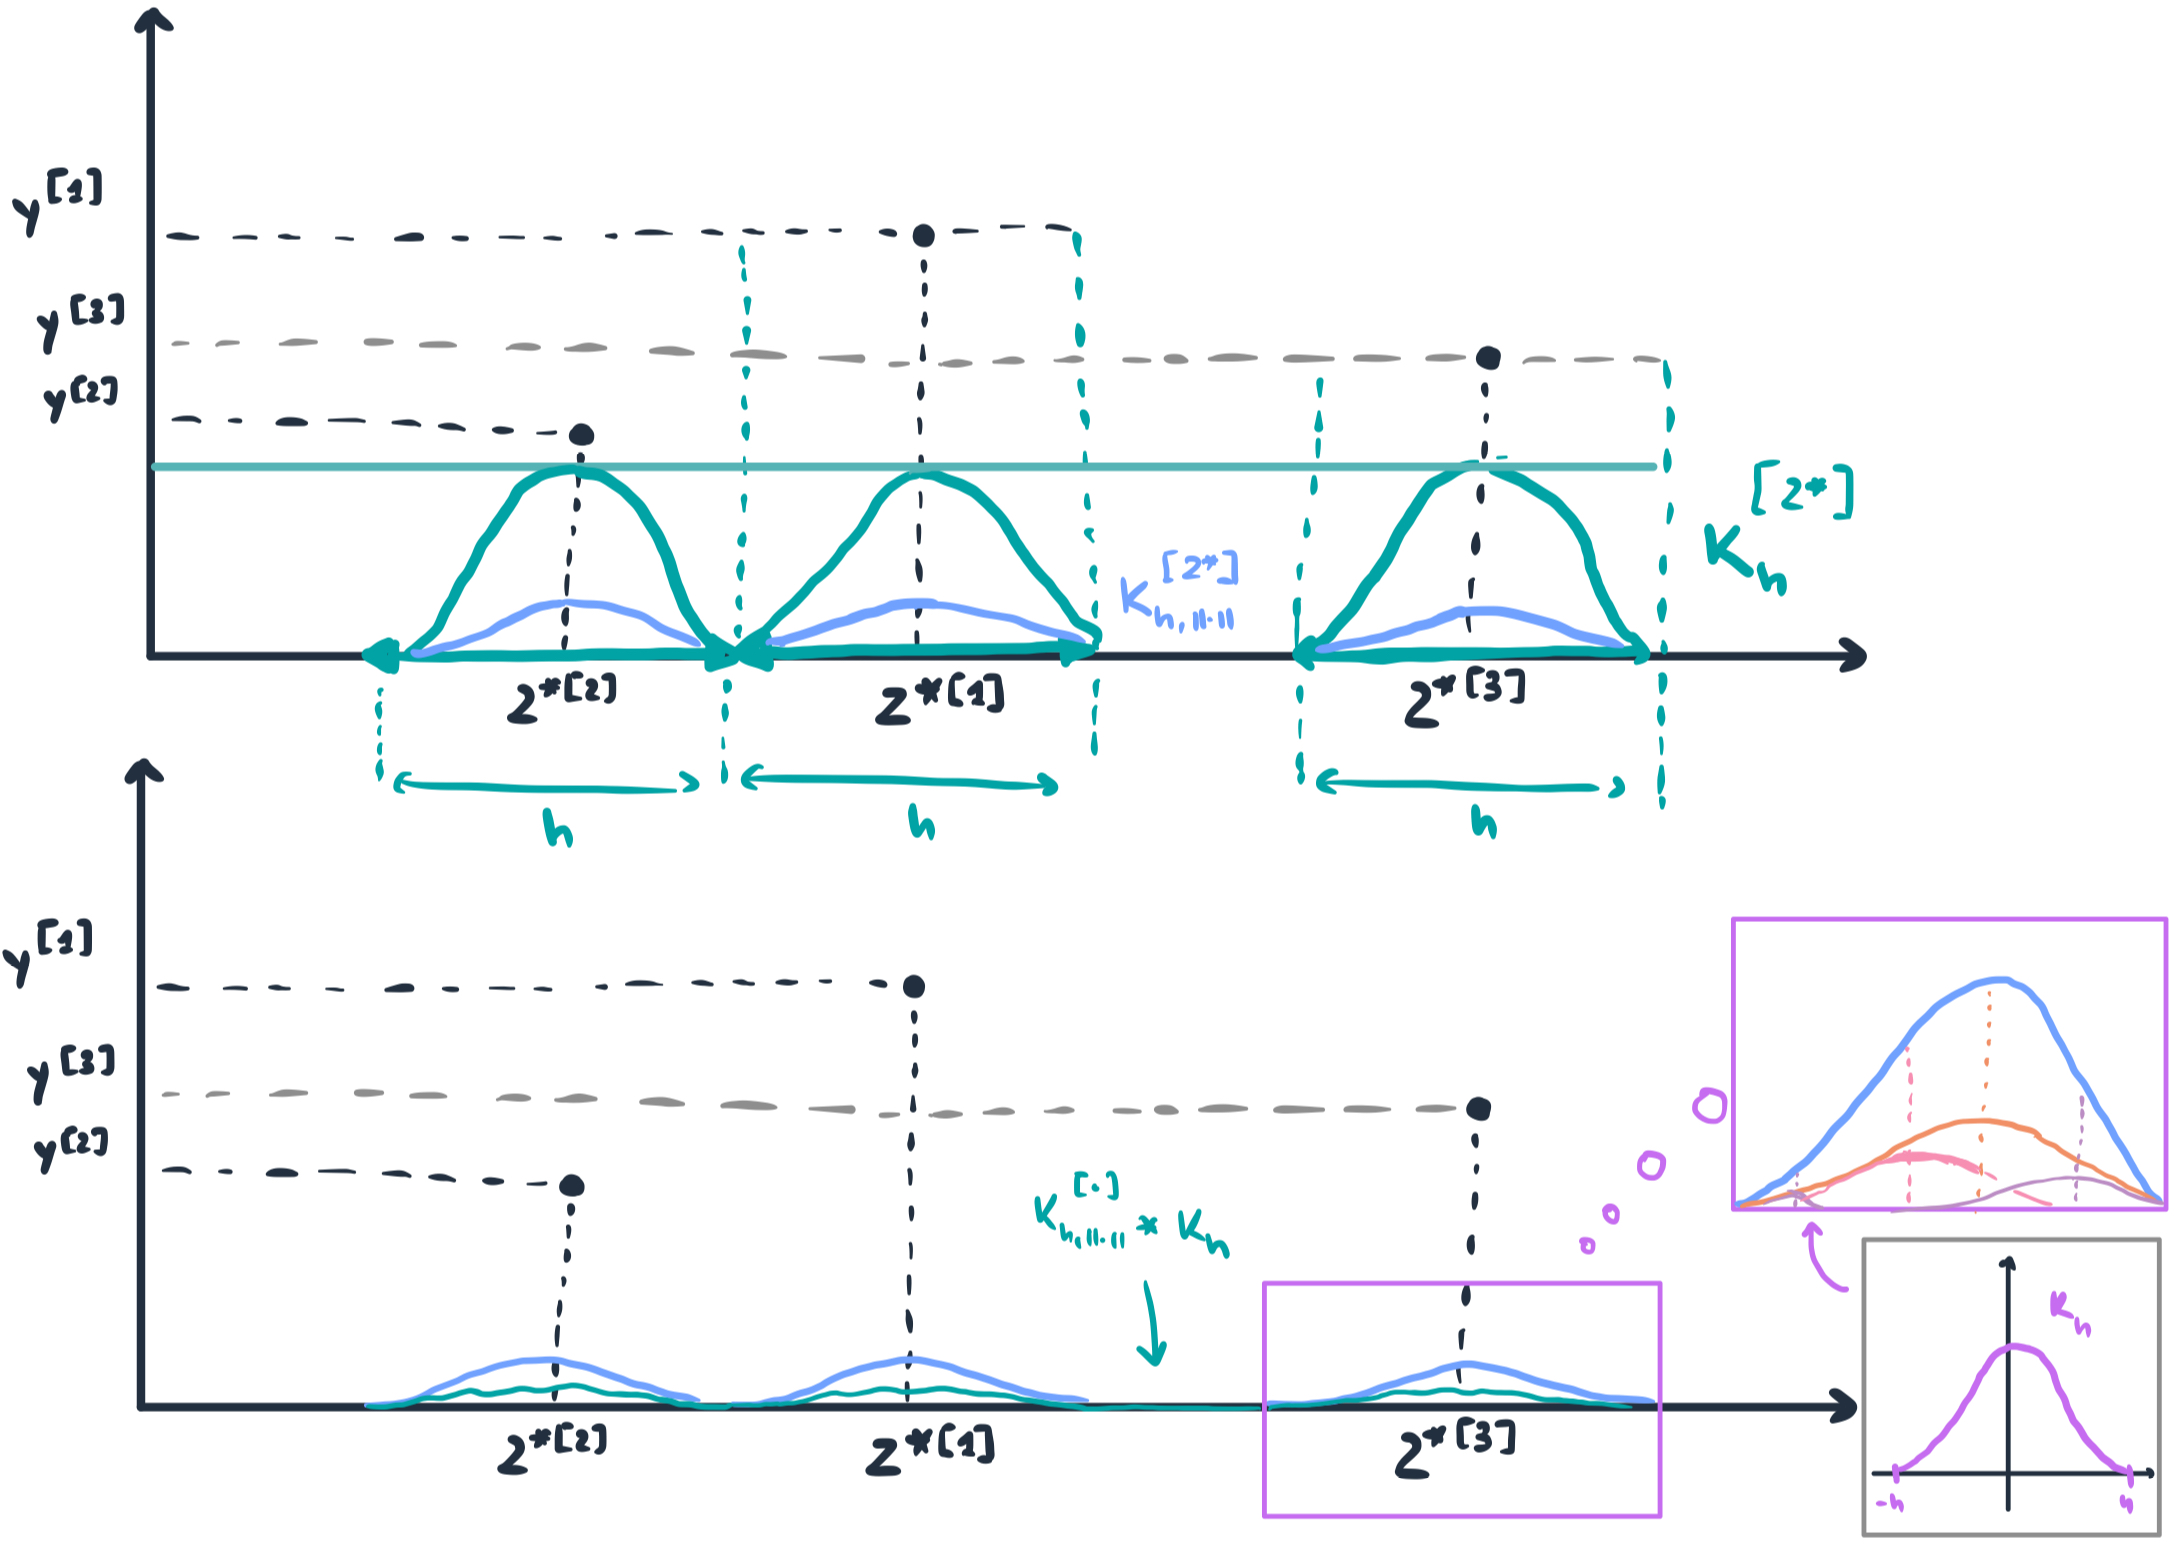
\includegraphics[width=0.75\textwidth]{Images/convo_kernel_interp.jpeg}
        \caption{Illustration de la convolution de $K_{h, \lVert \cdot \rVert}^{[\ \bullet \ ]}$ et $K_h$}
        \label{fig:convo_kernel_interp}
    \end{figure}

    On obtient ainsi des poids normalisés sur toutes les observations qui se basent sur le noyau de lissage de base $K_h$ que l'on a choisi.
    }

De façon plus formelle :
\begin{equation}
    \tilde K_h^\star(z, Z^*) =
    \displaystyle
    \frac{1}{2\pi h}
    \int 
    e^{-i\omega \frac{z-Z^*}{h}} 
    \cdot 
    \frac
    { 
        \phi_{
            K_{\, \lVert \, \bullet \, \rVert}^{[\,\int \,]}
        }
        (\omega \,, z\, \vert \, h) 
        \phi_K(\omega)
    }
    {
        \phi_u\left(\frac \omega h\right)
    }
    d\omega
\end{equation}\label{eq:norm_deconvolution_kernel}

où $\phi_{K_{\, \lVert \, \bullet \, \rVert}^{[\,\int \,]}}(\omega \,, z\, \vert \, h) = \int e^{i \omega \left(\frac{z-u}{h}\right)} K_{h, \lVert \cdot \rVert}^{[\, u \,]}(z)  \, du$ est la transformée de fourier selon les points de centrage (les $Z^*$ observés).

\subsubsection{Propriétés asymptotiques}

Le rapport de stage commençant à être long, nous ne détaillerons pas spécifiquement la méthodologie de cette section et nous renvoyons le lecteur à l'article de Han, Park \& Byeong (2018) \cite{han2018smooth} pour plus de détails. Nous allons juste mentionner les résultats principaux. En supposant que l'on dispose d'un contrôle du comportement de la fonction caractéristique de l'erreur de mesure dans les covariables en s'éloignant de $0$ : 

\begin{equation}
    \begin{array}{rcl}
        |\phi_V| &=& \underset{|t| \rightarrow \infty} O(|t|^{-\alpha})
        \\
        &\textsf{et}&
        \\
        |\phi'_V(t)| &=& \underset{|t| \rightarrow \infty}{O}\left( |t|^{-(\alpha+1)} \right) \textsf{ pour un }\alpha \geq 0
    \end{array}
\end{equation}

\noindent Le noyau proposé permet d'obtenir une estimation des fonctions $m_k$ dans le modèle $y = \sum_{k=1}^d m_k(z_k) + \varepsilon$ avec une vitesse de convergence \emph{optimale pour le problème de déconvolution en dimension $1$} sur l'intérieur du support de la densité $p_Z$, $I_h = \prod_{k=1}^d[2h_k, 1 -2h_k]$, en choisissant le bon $h$ (par validation croisée). Par exemple si $\alpha < 1/2$, la sélection du $h$ optimal    permet d'obtenir avec l'estimateur du backfitting:

\begin{align}
    \sup_{z \in I_h} \left| \hat m^\star_k(z) - m_k(z) \right| &\underset{\alpha < 1/2}= O_{\mathds P} \left( n^{- \frac{2}{5 + 2 \alpha} }\sqrt{\log n} \right)
    \\
    \sup_{z \in [0,1]} \left| \hat m^\star_k(z) - m_k(z) \right| &\underset{\alpha < 1/2}= O_{\mathds P} \left( n^{- \frac{2}{5 + 2 \alpha} } \right)
\end{align}

\noindent On peut alors utiliser le noyau de déconvolution normalisé pour l'estimation des fonctions de régression par un estimateur de Nadaraya-Watson dans le cadre d'un modèle additif en utilisant l'algorithme du Backfitting. 